% 4. CrossSection

% – Why is it relevant, what does the literature say

The section will present the results of different cross sectional analyses of the signal against the stock returns. Different portfolio sorts will be deployed to give the best possible view of the complete picture. Specifications of the different portfolio sorts are shown in Table \ref{tab:scenarioids}. 

The portfolio sortings will include results from both univariate and bivariate sortings, to illustrate the differences in taken either or both signals into account. Note, that the results in the unconditional analysis will be considering a more diverse set of portfolios to illustrate the choices made in the portfolio formation. 

This section is divided into a brief unconditional analysis, which will highlight the descriptive statistics of different portfolio sorts and evaluate the monotonicity in the returns of the portfolios. Following the unconditional analysis is the conditional analysis, which introduces additional external factors into the analysis, with an evaluation of the factor competition, priced risk factors, and explanatory power of the portfolios with the new factors. Lastly, I will illustrate the ex-post economic evaluation through looking at optimal allocation given allocation constraints and forming the efficient frontier.

%The portfolios ::: univariate on both variables -> which shows the most economic tendencies + bivariate sorting with both and arguments as to which sorting is best.


\subsection{Unconditional Analysis}

The descriptive statistics of the portfolios are great at providing an initial understanding of the formation. First I would like to compare two univariate portfolio sorts with the two different signals, so as to argue in combination with an economic motivation as to why I choose to have a bivariate sorting with the first sorting variable being the value of the implied volatility spread, and the second sorting variable being the change in the implied volatility spread. In addition to this I find it relevant to relate these two portfolios to a bivariate dependent portfolio sort. All of this is shown in Table \ref{tab:descr_stats_univariate_sortings}. 

\begin{table}[ht]
	\centering
	
	\caption[Descriptive Statistics, Univariate Sorting, 5 portfolios]{Descriptive Statistics of 5 Univariate Equal-sized Portfolios Sorted on the two Signals}
	\label{tab:descr_stats_univariate_sortings}
	
	\begin{subtable}[t]{0.65\textwidth}
		\caption[A]{Signal : Level of Implied Volatility Spread last trading day}
		\begin{tabular}{l|rrrrr}
			% latex table generated in R 4.1.2 by xtable 1.8-4 package
% Sat May 27 14:58:02 2023
stat & 1 & 2 & 3 & 4 & 5 \\ 
  \hline
Mean & -0.0254 & 0.0816 & 0.1775 & 0.2841 & 0.3915 \\ 
  Std & 3.2318 & 2.6529 & 2.4390 & 2.5787 & 3.0877 \\ 
  Skew & -0.5685 & -0.6762 & -0.2319 & -0.1191 & 0.0802 \\ 
  Kurt & 8.0285 & 7.8741 & 8.5110 & 7.9112 & 9.4463 \\ 
  Sharpe Ratio & -0.0079 & 0.0307 & 0.0728 & 0.1102 & 0.1268 \\ 
  
		\end{tabular}
	\end{subtable}
	
	\begin{subtable}[t]{0.65\textwidth}
		\caption[B]{Signal :  Change in Implied Vol Spread during last 7 days}
		\begin{tabular}{l|rrrrr}
			% latex table generated in R 4.1.2 by xtable 1.8-4 package
% Sat May 27 15:33:19 2023
stat & 1 & 2 & 3 & 4 & 5 \\ 
  \hline
Mean & 0.0435 & 0.1295 & 0.2047 & 0.2407 & 0.3438 \\ 
  Std & 3.1298 & 2.5518 & 2.4225 & 2.5979 & 3.0649 \\ 
  Skew & -0.3427 & -0.4585 & -0.2915 & -0.2710 & -0.0557 \\ 
  Kurt & 8.4224 & 7.2910 & 7.6734 & 7.7292 & 8.7931 \\ 
  Sharpe Ratio & 0.0139 & 0.0508 & 0.0845 & 0.0927 & 0.1122 \\ 
  
		\end{tabular}
	\end{subtable}
	
	\begin{subtable}[t]{0.55\textwidth}
		\caption[C]{Bivariate Sorting : first: level, second: change, Dependent}
		\begin{tabular}{l|rrrr}
			% latex table generated in R 4.1.2 by xtable 1.8-4 package
% Fri May 19 22:24:29 2023
stat & 1\_1 & 1\_5 & 5\_1 &  5\_5 \\ 
  \hline
Mean & -0.1003 & 0.0419 & 0.2928 &  0.4456 \\ 
  Std & 3.9400 & 3.6117 & 3.4557 &  3.5492 \\ 
  Skew & -0.2631 & -0.2679 & 0.3267 & 0.1873 \\ 
  Kurt & 9.1387 & 8.3976 & 9.2525 & 8.2882 \\ 
  Sharpe Ratio & -0.0255 & 0.0116 & 0.0847 &  0.1255 \\ 
  
		\end{tabular}
	\end{subtable}
	
	{\small Note: Table shows the descriptive statistics measured over the entire sample period. The options fullfill the conditions outlined in Section \ref{section:data}, the implied volatility spread is weighted by open interest in every combination of date and stock, and the portfolios are equal-sized and have value-weighted returns. ScenarioIDs are 1, 10 and 2 respectively.}
\end{table}

I notice, first and foremost, that the mean return show a larger difference between the first and last portfolio in the first subplot (the portfolios based on the value of the implied volatility spread) than those of the second subplot (with the portfolios sorted on the change in implied volatility spread). The standard deviation, kurtosis and skewness seem approximately the same, and as a natural effect from this, the Sharpe Ratio shows approximately the same pattern as the returns, with both higher and lower levels obtained in the sorting based on level. 

When I look further down at the dependent bivariate portfolio sorting and compare the descriptive statistics of the 'corner'\footnote{The 'corners' are just the portfolios in the intersection between the first and last portfolios of the two sorting variables.} portfolios with two univariate portfolio sets, I note that the returns show more variance, but also that the standard deviation of the returns seem in general to be higher. Furthermore, the skewness is also higher, but the kurtosis seems at the same level. Of course, all the portfolios of the bivariate sorting has not been reported here to provide a more concise overview.

The distributions of the returns are showing a close-to normal distribution. The mean is near 0, the strandard deviation is varying across the portfolios, but seems to be centered around 3, the skewness is within $-2$ and $2$\footnote{According to \cite{byrne2013structural} a rule of thumb is that a skewness between $-2$ and $2$, and kurtosis between $-7$ and $7$ means the data is normally distributed.}, and the kurtosis is around 8, however, this is a little high to fall within the boundaries of a normal distribution. 

\begin{figure}[ht]
	\centering
	\caption[Mean Returns Across Bivariate Sorting]{Plot of the mean weekly returns of Bivariate Portfolio Sorting}
	\label{fig:mean_returns_bivariate}
	
	\begin{tabular}{cccc}
		\subfloat[Bivariate Sorting with Level and Change]{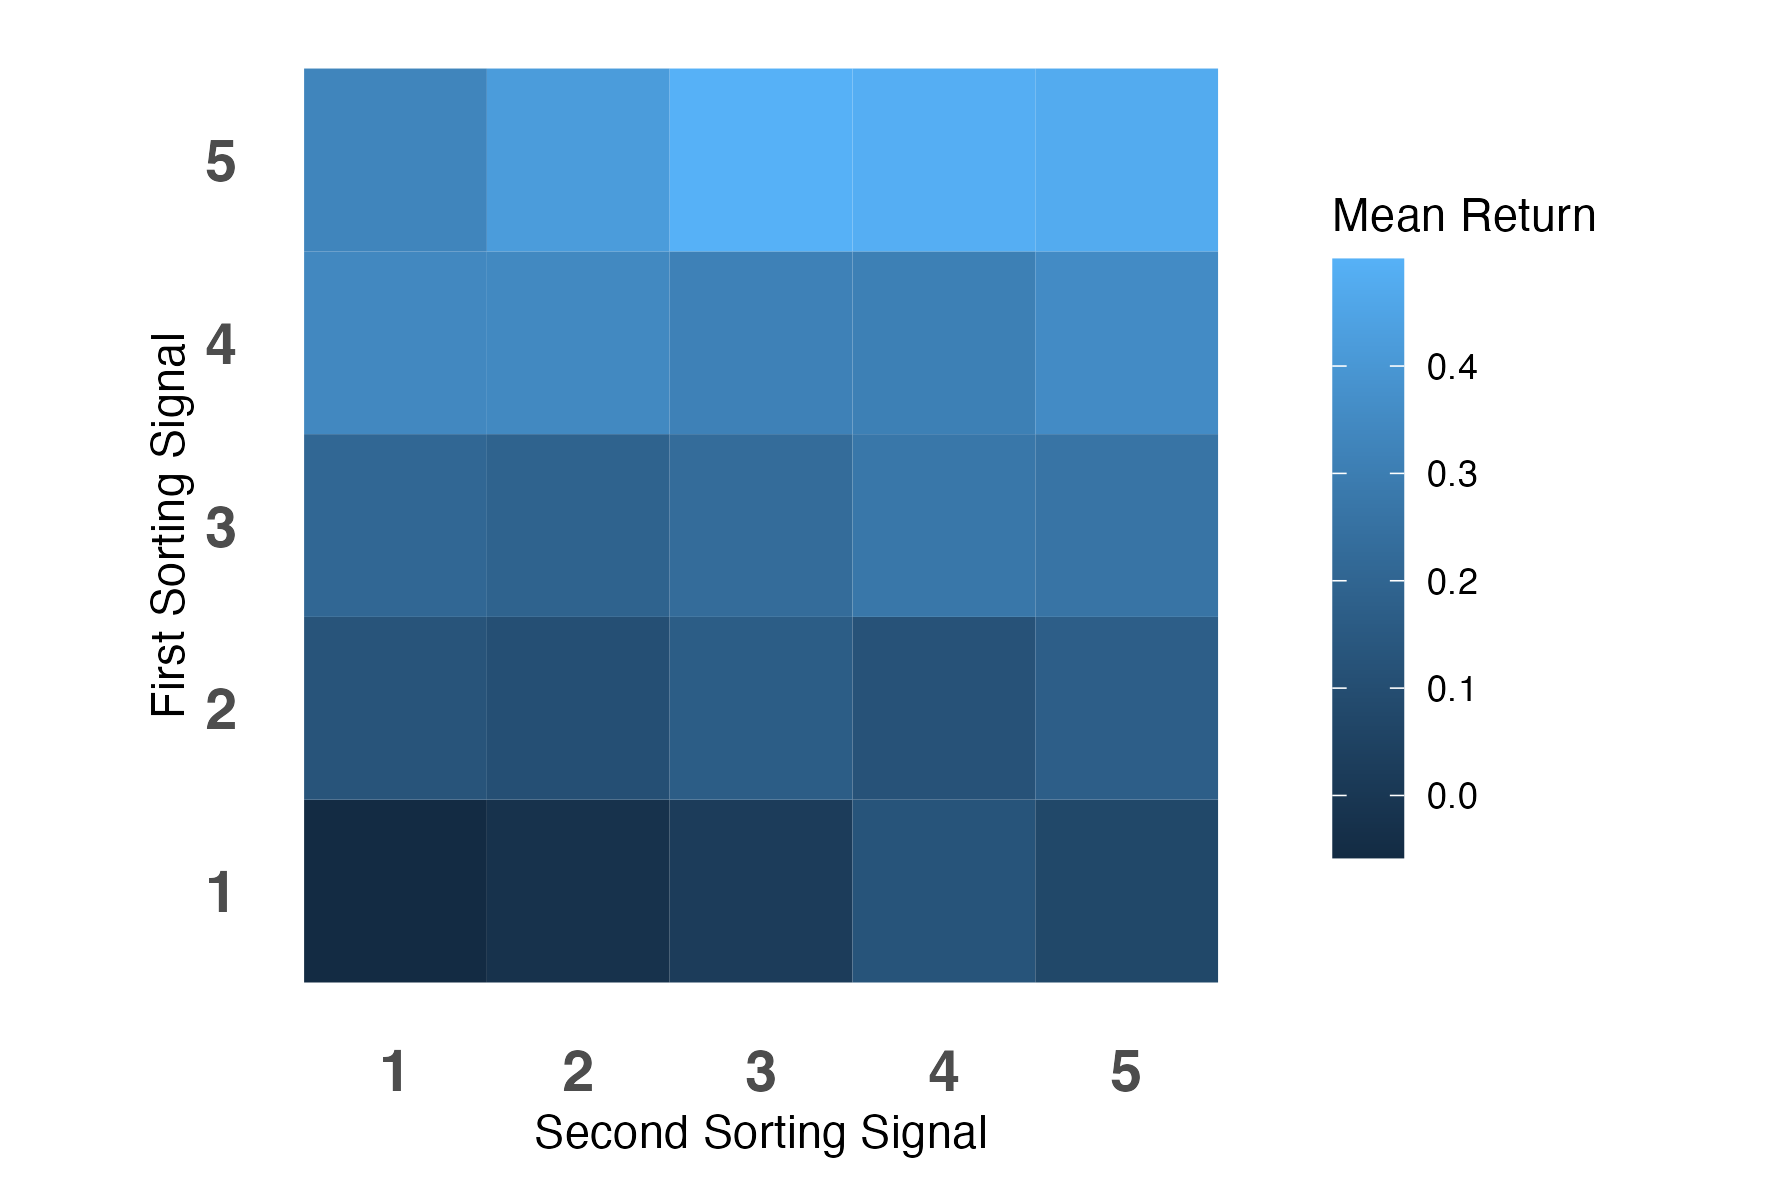
\includegraphics[width=0.45\textwidth]{./Plots/meanreturns_entireperiod_simple_2.png}} &
		\subfloat[Bivariate Sorting with Change and Level]{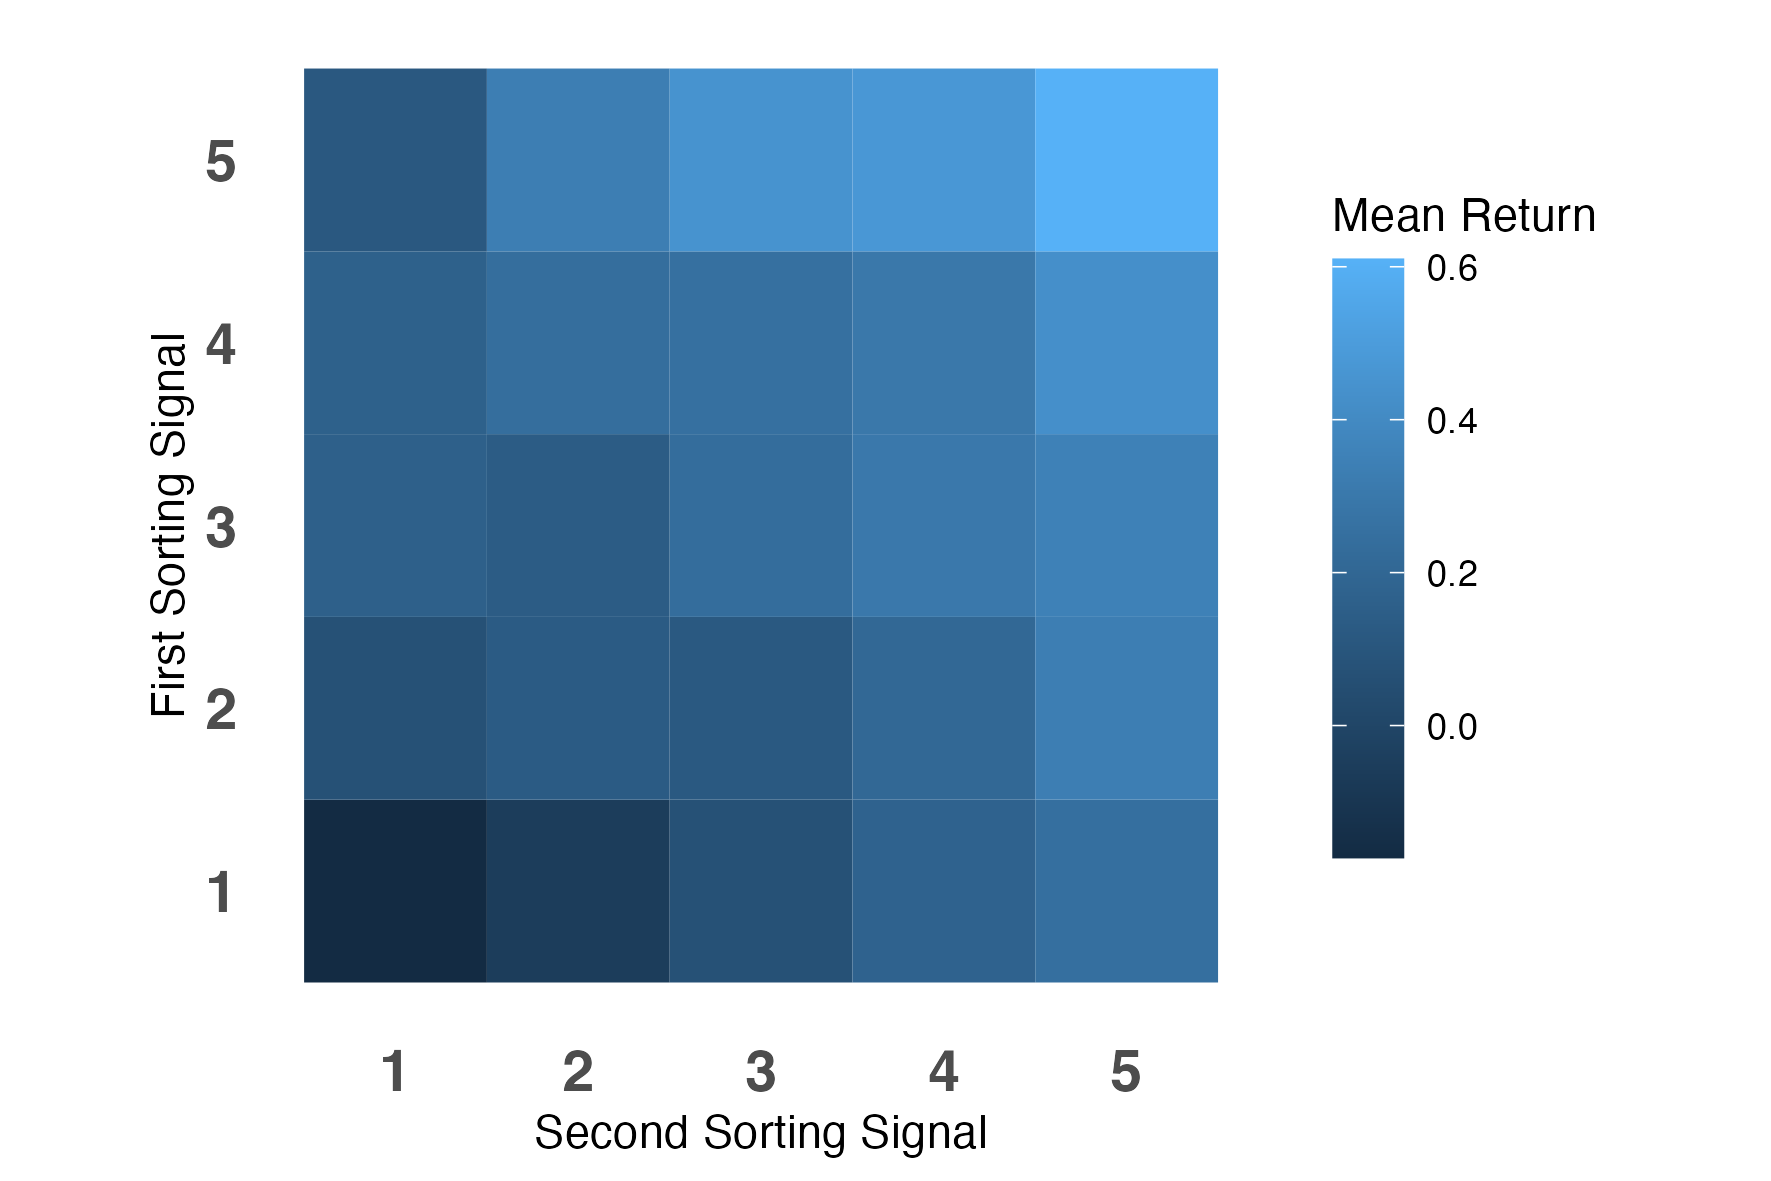
\includegraphics[width=0.45\textwidth]{./Plots/meanreturns_entireperiod_simple_18.png}} \\
	\end{tabular}

	{\small Note: Figure shows the mean weekly excess return over the entire sample period in percentage. Both sortings are dependent. The scales of the two plots differ, and subplot (B) has a wider scale. The returns are value-weighted. ScenarioID is 2 and 18 respectively.}
\end{figure}

To illustrate the dynamics in the bivariate portfolio sorting, the mean returns are portrayed in Figure \ref{fig:mean_returns_bivariate}. In subplot (A) there is a clear pattern of the biggest variation in mean return coming from the first sorting which is the level of the implied volatility. Subplot (B) shows a more symmetric pattern, but it still has a tendency of in general having a higher mean return in group 5 of the level sorting. As these scenarios have the level of the implied volatility as the axis of primary variance, it makes sense to focus at the level of the implied volatility spread compared to the change and use this as a signal, as both the economic arguments and patterns of mean returns support this. 

In the following, I will focus on a bivariate sorting with the level of the implied volatility spread, and the recent change in the implied volatility spread as the second sorting factor. The sorting will be dependent, to ensure that the portfolios will be equal-sized throughout the sample period. All returns are value-weighted\footnote{The choice of value-weighted vs. equal-weighted is elaborated upon in the following paragraph.}. In most cases, a focus will be on the 10 times 10 portfolios as they provide the most sensitive factor, but when it makes sense a smaller set of portfolios with the same choices will be shown. The 10 times 10 portfolios have a ScenarioID of 9, the smaller set of 5 times 5 has a ScenarioID of 2 and the last set of 3 times 3 with a split of 30\%, 40\% and 30\% has a ScenarioID of 14. 
% PRIMARY = 9, secondary = 2, tjertiary = 14

\begin{table}[ht]
	\centering
	
	\caption[Monotonicity Tests]{Three different Monotonicity Tests}
	\label{tab:monotonicity_tests_9}
	
	\begin{tabular}{l|rrrr}
		% latex table generated in R 4.1.2 by xtable 1.8-4 package
% Sat May 27 15:23:49 2023
category & monoton\_up & monoton\_down & Wolak & Bonferroni \\ 
  \hline
increasing & 0.0000 & 1.0000 & 0.9930 & 1.0000 \\ 
  decreasing & 0.0000 & 1.0000 & 0.7400 & 1.0000 \\ 
  
	\end{tabular}
	
	{\small Note: Table shows p-values for three different monotonicity tests, including the \cite{patton2010monotonicity} with both a test for increasing and decreasing monotonicity, and two selected others. ScenarioID is 9.}
	
\end{table}

\textbf{Monotonicity} For the monotonicity test of the portfolios, the diagonal set of portfolios are evaluated against eachother\footnote{This is due to the function deployed in the scripts are only capable of considering 15 portfolios at a time, so to make the analysis coherent across portfolios formations, this decision was taken.}. For the abovementioned portfolio set of 10 times 10 bivariate portfolio split, the diagonal portfolios' return are clearly increasing in the value of the level and of the change throughout the entire sample period. This can be seen in Table \ref{tab:monotonicity_tests_9} through the p-value of monoton-up is approximately 0, which means we reject the null-hypothesis of no monotonicity between the returns, as outlined in Equation \ref{eq:monoton_test}. The remaining two tests have a null hypothesis of a monotonic relation between the portfolios, and they both provide a fairly high p-value, which clearly indicates that they cannot reject the monotonic relationship between the return of the portfolios. Based on this I can conclude, that not only do I see a positive correlation between the implied volatility spread and the returns, but I also see it across most of the periods and across the portfolio formations. 

\textbf{Cumulative Returns} Inspecting the cumulative returns of the portfolios in Figure \ref{fig:cumula_returns_2}, and limiting it to scenarioID 2, which has a 5 times 5 bivariate sorting with the same characteristica as scenarioID 9, I can clearly see that the last group in the first sorting dimension provides the highest cumulative returns. The COVID-19 uncertainty hit all of the portfolios, but especially the last portfolio (5\_5) seems to recover fast and provide an even steeper climb in the returns afterwards.

\begin{figure}
	\centering
	\caption[Cumulative Weekly Returns]{Cumulative Simple Weekly Returns, over entire sample period}
	
	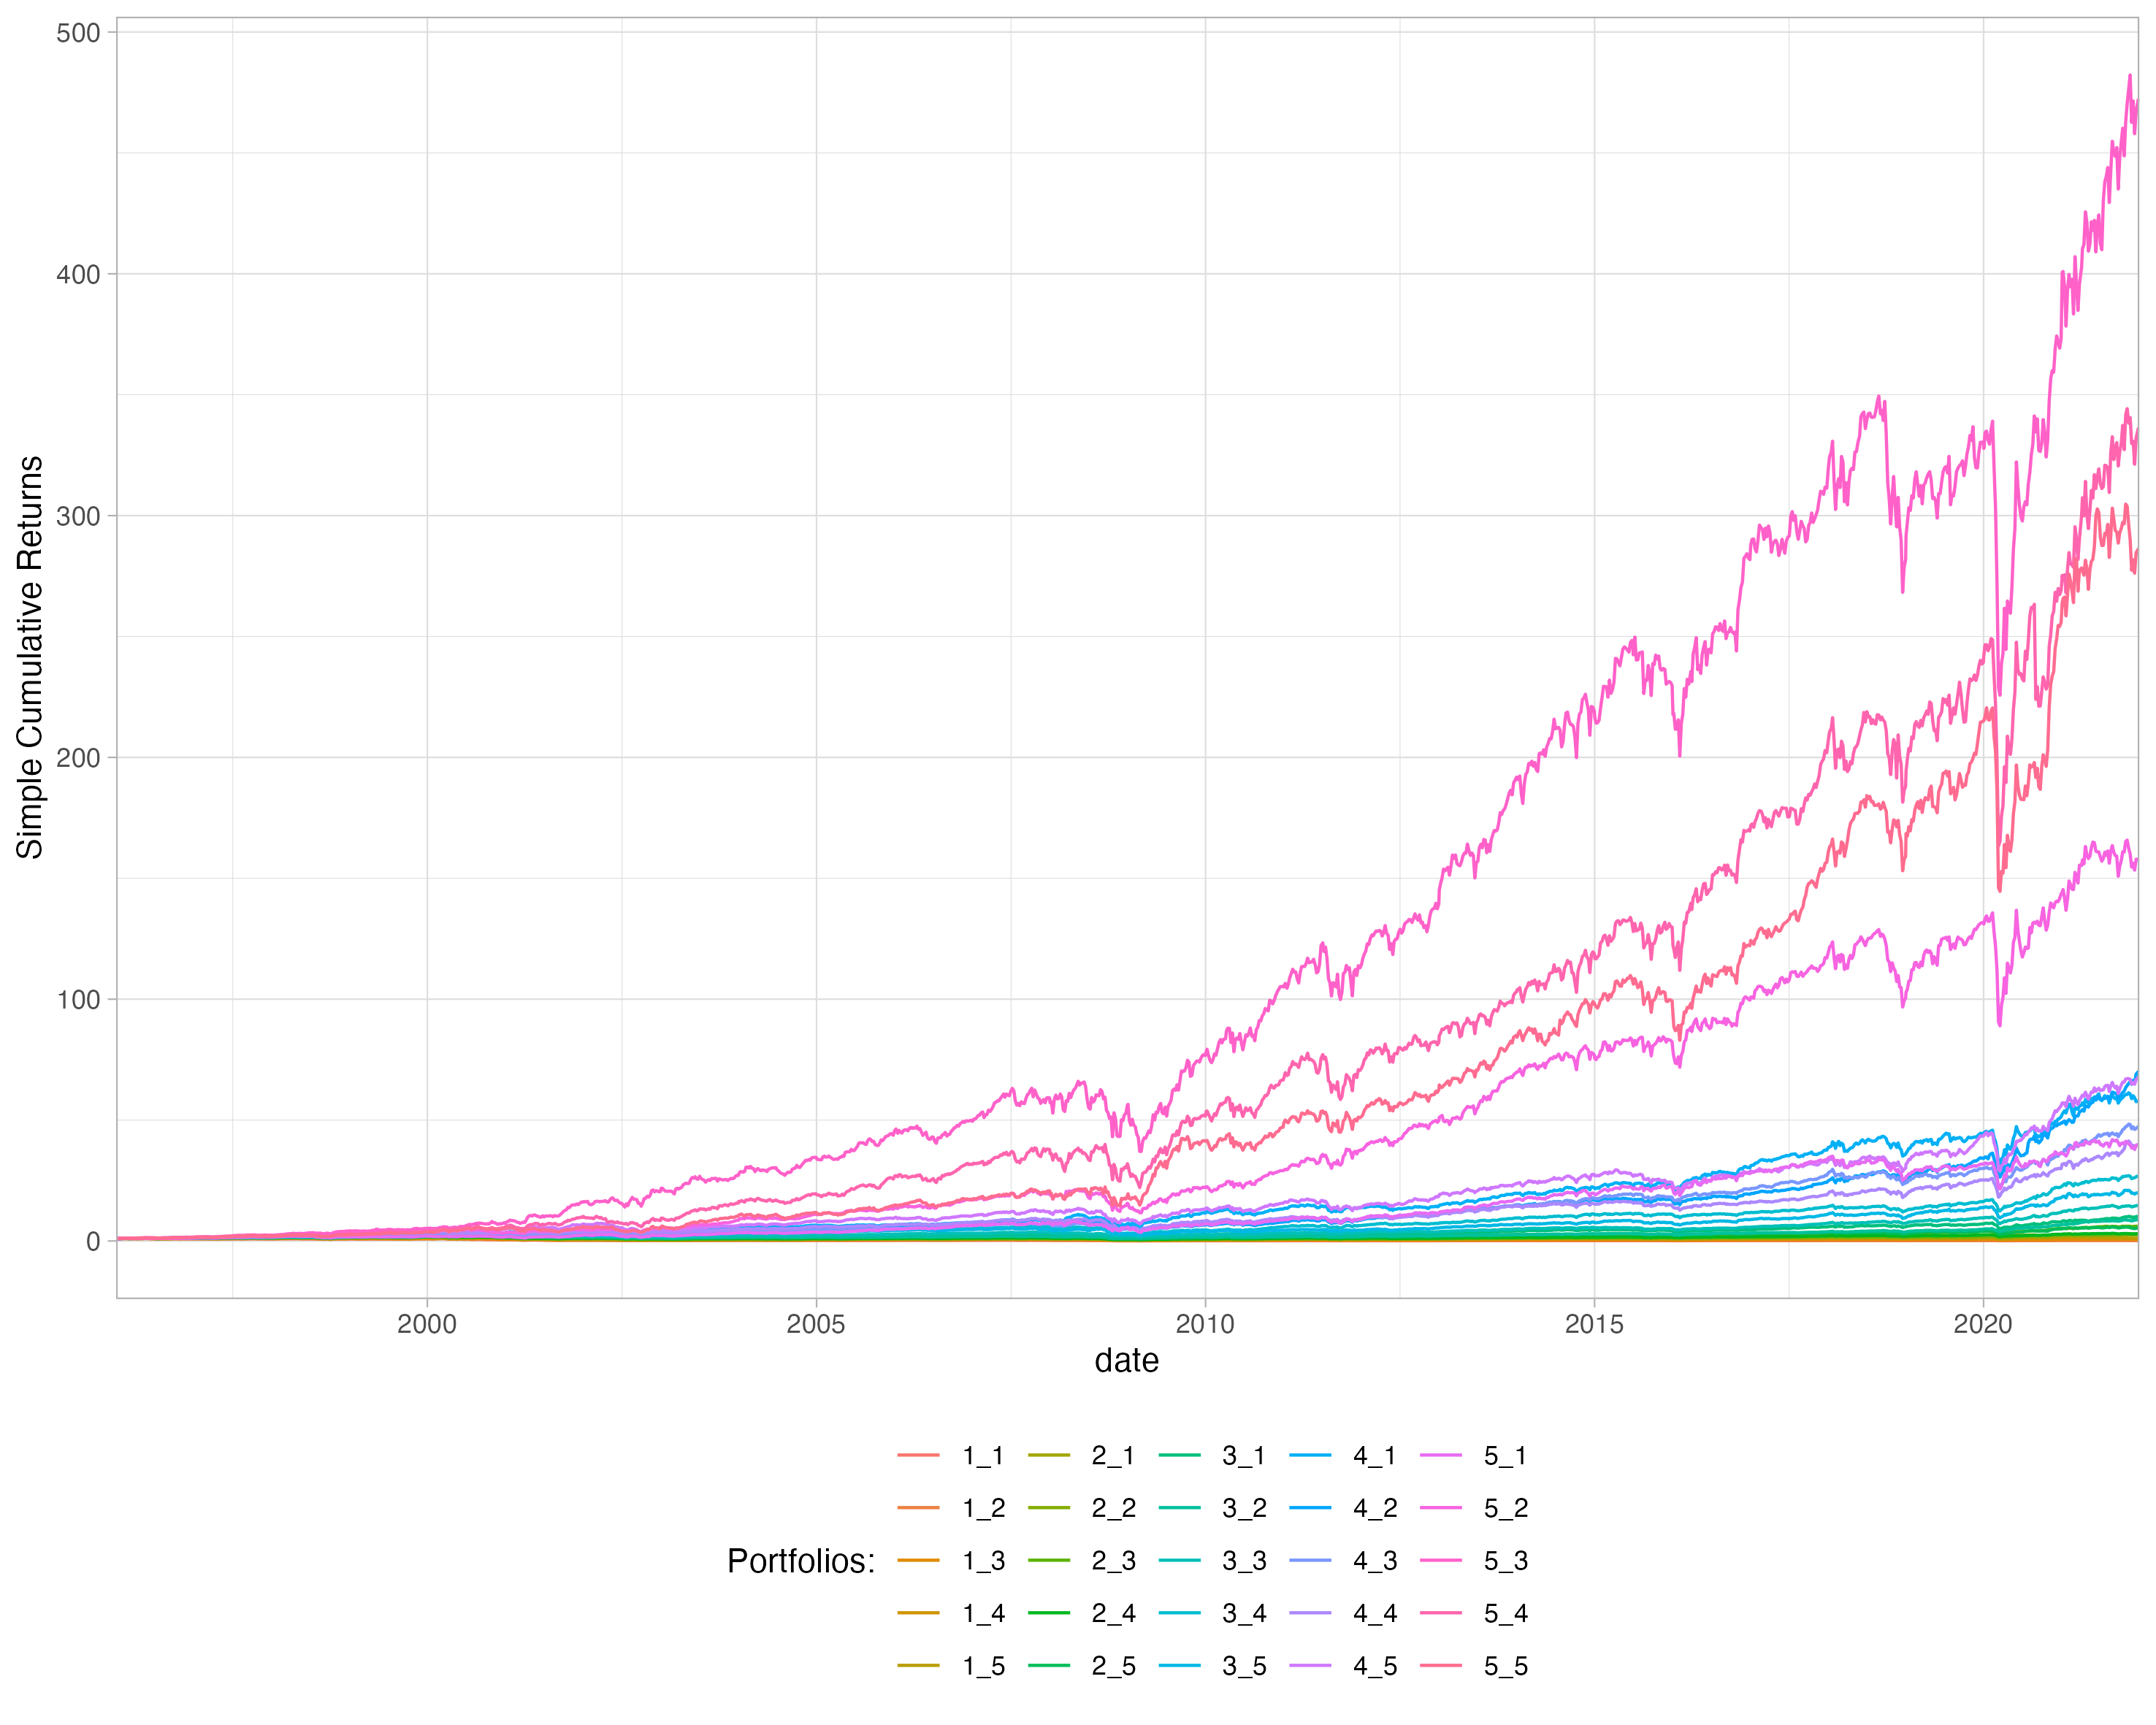
\includegraphics[width=0.95\textwidth]{./Plots/cumulativereturns_entireperiod_simple_2.png}
	\label{fig:cumula_returns_2}
	
	{\small Note: The cumulative returns are calculated as a simple cumulative product of the return over the entire sample period. The ScenarioID is 2.}
	
\end{figure}

\textbf{Comparing Value-Weighted and Equal-Weighted Returns} In this short note on the use of value-weighted returns in the portfolios, I will compare the already shown portfolios with their equivalent equal-weighted portfolios, so any discrepancies or doubts regarding the significance of the results can be disproved.

%SHOW SOME TABLES HEEEEEERE

% compare 1, 2 and 10 to 15, 16 and 17


\subsection{Conditional Analysis}

Following the unconditional analysis of the portfolios, I will now expand the analysis to include factors from the literature, to evaluate if the long-short zero-net-investment factor formed on the portfolios has a statistical significant risk premium, and if this factor is explained by some common factors from the literature. 

The subsection will start with the spanning regressions to evaluate the factor competition, then move on to Fama-Macbeth regressions of both time-invariant and time-variant versions with differing amount of extra factors, to see the effect and evaluate any changes in the coefficients. To supplement the Fama-Macbeth regressions, the three-step procedure is then implemented, and the results of the risk premia estimations as well as the strength of the models are expanded upon. Lastly I will do a brief analysis of a pooled regression with the relevant portfolios regressed upon dummies for the portfolio index and the different factors considered up until then.

\subsubsection{Factor Competition}

The factor competition is a fairly simple regression of the different factors included regressed upon the remaining factors. I do this to see if each factor is explained by the remaining and therefore considered irrelevant.

As shown in subsection \ref{subsec:forming_factors} in Figure \ref{tab:factor_competition_impl} the intercepts of factor formed on different univariate portfolios show fairly consistently that the remaining factors do not explain the average of the long-short factor formed on the level of the implied volatility spread. It is, however, interesting to see if both the long-short factor and the diagonal version have intercepts different from zero. 

\begin{table}[ht]
	\centering
	\caption[Factor Competition against FF5]{Factor Competition of Long-Short Portfolios against FF5 factors}
	\label{tab:factor_competition_9}
	
	{\small
		\begin{tabular}{l|llllllll}
			% latex table generated in R 4.1.2 by xtable 1.8-4 package
% Sat May 27 15:23:54 2023
Dep. Variable & Intercept & IMPVOL & IMPVOL\_D & MKT\_RF & SMB & HML & RMW & CMA \\ 
  \hline
IMPVOL & 1.04  (***) &  & 0.04 & 0 & -0.07 & 0.12 & -0.08 & -0.08 \\ 
  IMPVOL\_D & 0.54  (***) & 0.03 &  & 0.06 & 0.11 & -0.04 & 0.22  (*) & 0.14 \\ 
  MKT\_RF & 0.22  (***) & 0 & 0.02 &  & 0.14  (**) & 0.27  (***) & -0.55  (***) & -0.5  (***) \\ 
  SMB & 0.03 & -0.01 & 0.01 & 0.05  (**) &  & -0.08  (**) & -0.34  (***) & 0.06 \\ 
  HML & -0.05 & 0.02 & -0.01 & 0.11  (***) & -0.09  (**) &  & 0.2  (***) & 0.6  (***) \\ 
  RMW & 0.1  (**) & -0.01 &  0.02  (*) & -0.12  (***) & -0.22  (***) & 0.1  (***) &  & 0.2  (***) \\ 
  CMA & 0.04 & 0 & 0.01 & -0.07  (***) & 0.03 & 0.2  (***) & 0.13  (***) &  \\ 
  
		\end{tabular}
		
	}
	{\small Note: Table shows the coefficients of the regressions according to Equation \ref{eq:factorcompetition}. The regression span the entire sample period and consists of weekly returns. The significance of  the coefficients are coded according to the p-value: $0 < (\ast\ast\ast) < 0.001 < (\ast\ast) < 0.01 < (\ast) < 0.05$. The scenarioID is 9.}
	
\end{table}

In Table \ref{tab:factor_competition_9} the factor competition coefficients are shown. The FF5 factors are clearly having an effect upon eachother, but their relation to the estimated factors here are statistically not different from zero. Furthermore, a surprising observation is that the coefficients between the implied volatility spread factor and the diagonal version is not significant, which means that the two sorting factors are complimenting eachother in the formation. This will be explored further in the following sections. 

Note that the results in this subsection is not directly comparable to the ones reported in \cite{fama2015five}, as the frequency is different. These results are based on a slightly higher frequency of weekly returns compared to the monthly returns which constituents the main focus of their article.

To evaluate the factors against more than just the FF5 factors, I have included results in Table \ref{tab:factor_competition_9_ALL} of the factor competition with all factors outlined in Section \ref{section:empirical} and this provides the same picture as above, with the intercept of the implied volatility spread factors being statistical significant different from zero at a fairly high degree and only a few of the added factors have coefficients different from zero at 10\% certainty. Based on this, I deem it relevant to use this factor in the further analysis, as it provides a new dimension of variability not captured by the remaining factors.

\subsubsection{Fama-Macbeth Regressions}

The Fama-Macbeth regressions are made to get an estimate for the risk premium. LS denotes the long-short factor, and LSD denotes the diagonal version. The first two sets of regressions will be based on the portfolios from ScenarioID 9 with a bivariate dependent portfolio sort of 10 times 10 portfolios sorted on level and then change in the implied volatility spread. The factors are limited to the long-short factors of the portfolios and on the median level of the implied volatility spread within each portfolio at each point in time. 

\begin{table}[h]
	\centering
	
	\caption[Fama-Macbeth Regression, One Factor]{Fama-Macbeth Regressions, using Median of the signal as Factor}
	\label{tab:fm_simple_9}
	
	\begin{subtable}[t]{0.55\textwidth}
		\caption[C]{Time-Invariant}
		\begin{tabular}{l|rrrr}
			% latex table generated in R 4.1.2 by xtable 1.8-4 package
% Sat May 27 15:23:55 2023
term & gamma\_hat & gamma\_hat\_se & tstat \\ 
  \hline
(Intercept) & 0.1584 & 3.5398 & 0.0448 \\ 
  LS & 1.3958 & 4.5724 & 0.3053 \\ 
  LSD & 0.7398 & 4.1664 & 0.1776 \\ 
  median & -0.0006 & 0.0621 & -0.0090 \\ 
  
		\end{tabular}
	\end{subtable}
	
	\begin{subtable}[t]{0.55\textwidth}
		\caption[C]{Time-Variant, rolling window = 52 weeks}
		\begin{tabular}{l|rrrr}
			% latex table generated in R 4.1.2 by xtable 1.8-4 package
% Sat May 27 15:23:59 2023
term & gamma\_hat & gamma\_hat\_se & tstat \\ 
  \hline
(Intercept) & 0.1747 & 2.7459 & 0.0636 \\ 
  LS & 0.6457 & 4.7647 & 0.1355 \\ 
  LSD & 0.4632 & 4.4420 & 0.1043 \\ 
  median & 0.0007 & 0.0156 & 0.0429 \\ 
  
		\end{tabular}
	\end{subtable}
	
	{\small Note: The regression span the entire sample period and consists of weekly returns. The rolling window used for subtable (B) has a lenght of 52 weeks. The scenarioID is 9. %The significance of  the coefficients are coded according to the p-value: $0 < (\ast\ast\ast) < 0.001 < (\ast\ast) < 0.01 < (\ast) < 0.05$.
	}
	
\end{table}

\textbf{Simple and Time Invariant} Starting with the time-invariant version, in which I assume that the exposure of the portfolios against the included factors are constant in the sample period and the risk premium is also constant. The results are shown in Table \ref{tab:fm_simple_9}. The coefficients are all insignificant, as the t-statistics for each and every one of them are less than 0.5 in absolute value. Furthermore, the median actually has a negative coefficient, which seems at odds with the conclusions from above, where I identified a clear positive correlation between the mean returns of the portfolios and the sorting variable in both the monotonicity tests and the descriptive statistics. This could, however, be due to the LS factor catching the increasing effect and then the median correcting for the less extreme variations in the middle portfolios.

\textbf{Simple and Time Variant} Shifting the focus to the second part of Table \ref{tab:fm_simple_9}, the coefficients for the factors have nearly halfed in size and are even further from being significantly different from zero. The median has, however, now a more intuitive positive coefficient. 

The Fama-Macbeth regressions do require, however, that all priced factors are included in the regression. Therefore, I will expand the analysis to take FF5 factors into account, and hope to gain some more meaningfull coefficients (and risk premiums) from this\footnote{The reason for the exclusion of the Open Asset Pricing Factors is the lower frequency of their availability, as they are only reported on a monthly basis.}.

\begin{table}[ht]
	\centering
	
	\caption[Fama-Macbeth Regression, FF5]{Fama-Macbeth Regressions, using FF5}
	\label{tab:fm_FF5_9}
	
	\begin{subtable}[t]{0.55\textwidth}
		\caption[C]{Time-Invariant}
		\begin{tabular}{l|rrrr}
			\input{./Tables/fm_results_timeinvariant_FF5_9.tex}
		\end{tabular}
	\end{subtable}
	
	\begin{subtable}[t]{0.55\textwidth}
		\caption[C]{Time-Variant, rolling window = 52 weeks}
		\begin{tabular}{l|rrrr}
			\input{./Tables/fm_results_timevariant_FF5_9.tex}
		\end{tabular}
	\end{subtable}
	
	{\small Note: The regression span the entire sample period and consists of weekly returns. The ScenarioID is 9.}
	
\end{table}

\textbf{FF5 and Time Invariant} To accommodate the requirements of the Fama-Macbeth regression framework, I have added five additional factors to the regression. The results are shown in Table \ref{tab:fm_FF5_9}, and as with the results of the more limited regression, none of the coefficients are statistically significantly different from zero. And additionally, the market factor seems to have an estimated negative risk premium. This is at odds with the expectation, as the market risk premium should be positive as the market excess return has been positive on a historic basis and is positive in the estimation made by \cite{giglio2021asset}. 

\textbf{FF5 and Time Variant} Shifting the focus to the time-variant version of the Fama-Macbeth regressions, two very large risk premium estimates stand out. It seems that the coefficients have been affected by some of the data missing or being very alike in value resulting in the OLS estimator finding an unlikely high number. The standard errors are equally as large and the resulting t-statistic is within the same range as the remaining. This might also be a sign of colinearity issues between the factor and its diagonal version, which also makes sense given that the risk premium of the diagonal version is suddenly estimated to be negative. The remaining coefficients have the expected sign, as all factors have a positive risk premium. 

All-in-all the results from the Fama-Macbeth regressions left no clear conclusion, as the risk premiums were insignificant, which is in contrast to results from the literature. I will go forward with the three-step procedure to see if this approach can identify the underlying variations of the portfolios and map this to the factors included.

\subsubsection{Three-Step Procedure}

The three-step procedure was introduced to remove the omitted variable bias and to exploit the deployment of principle components analysis to find the main dimensions of the variance of the returns. 

The returns set I am deploying here is the 100 portfolios estimated in Scenario 9, with bivariate dependent portfolio sorting and the set of 100 portfolios from Kenneth French's Library based on size and value. Note that no other portfolios are considered, even though the authors argue for the inclusion of portfolios exposed to all asset classes.

The first step is to estimate the main points of variance in the returns through principal components analysis. Using the cost function outlined in Section \ref{section:empirical} in Equation \ref{eq:tp_cost} and results in an optimal choice of relevant dimensions to be three for this analysis. The explained variance of each of the first 25 principal components are shown in Figure \ref{fig:explainedvariance_9}, where the first principal component clearly outperforms the remaining. The choice of the first three principal components to be used further in the analysis is, of course, subject to critique and I will therefore include the results of 1 principal component up until the optimal plus two. This way we can see the robustness in the coefficients across different choices for the principal components.

\begin{figure}[h]
	\centering
	\caption[Proportional Explained Variance]{Proportional Explained Variance of Principal Components}
	\label{fig:explainedvariance_9}
	
	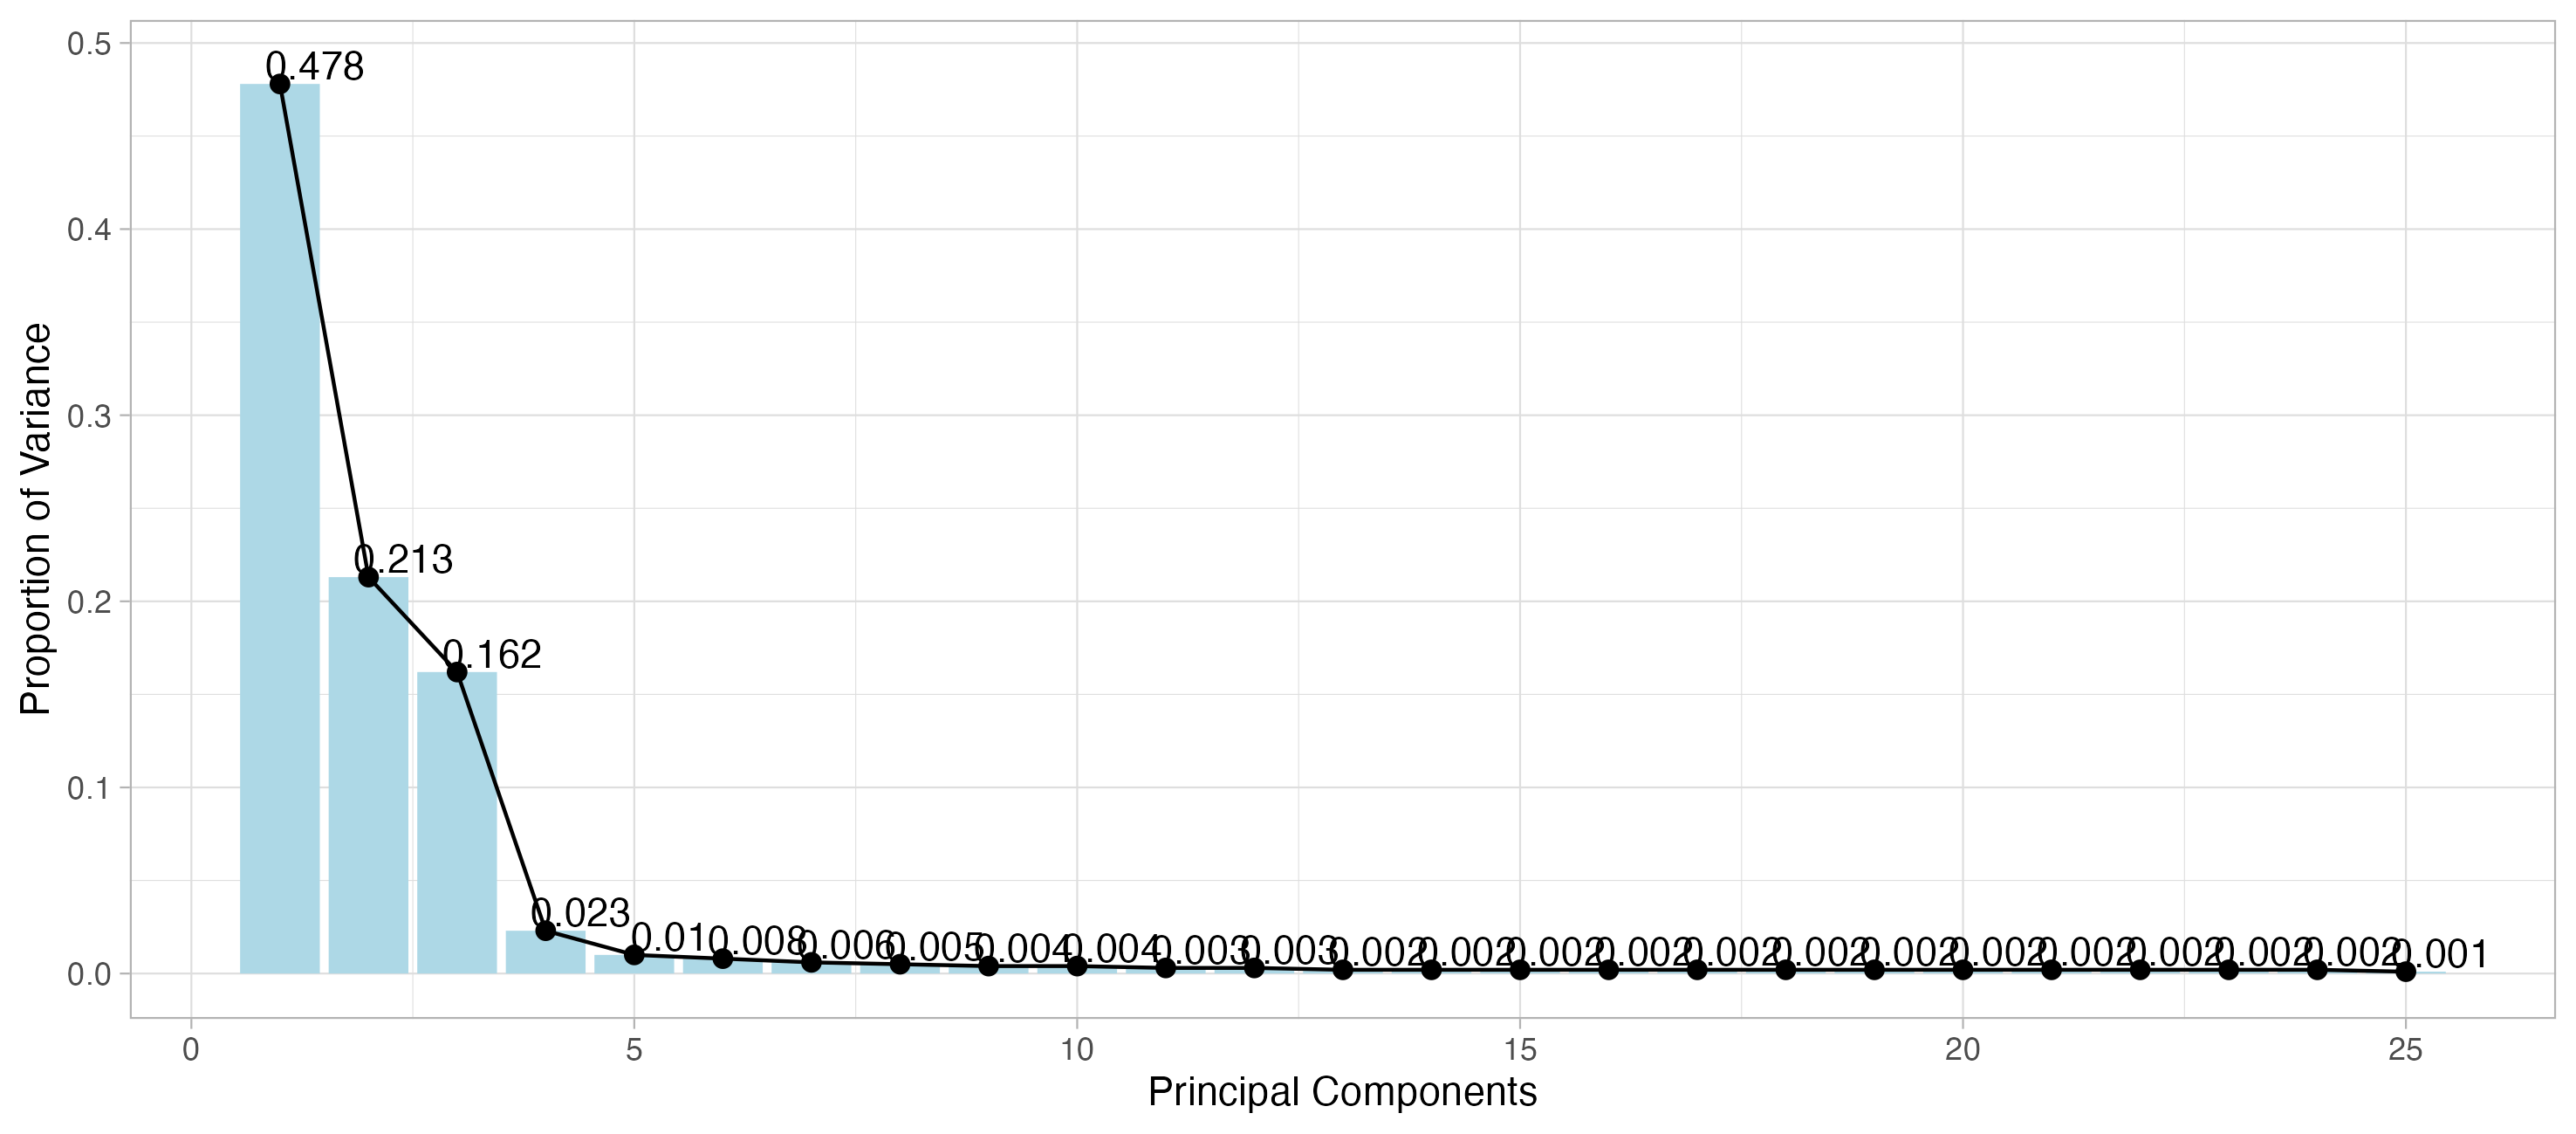
\includegraphics[width=0.85\textwidth]{./Plots/principalcomponents_proportionvar_9.png}
	
	{\small Note: the figure shows the explained proportion of variance of each principal component of the set of returns of 100 portfolios from ScenarioID 9 and 100 size-value portfolios from Kenneth French.}
\end{figure}

In Table \ref{tab:tp_results_9} the risk premia estimates are reported along with their statistical significance for each choice of principal components. As the optimal value for $\hat{p}$ is 7, I note that only the long-short factor based on the portfolios is significant, and that only at a 5\% level. The factor stays somewhat significant through the robustness versions, as can be seen in column 8 and 9. The results from the regression seems robust to including more principal components, as the coefficients and significance levels are fairly constant across the different runs. None of the remaining included factors besides the long-short factor based on the portfolios are significant, which could be explained by the limited set of portfolios used in the regression, as \cite{giglio2021asset} argues that a variety of different portfolios should be included in the original estimation. 

\begin{table}[h]
	\centering
	
	\caption[Three-Step Procedure, Coefficients]{Coefficients from the Three-Step Procedure, using FF5}
	\label{tab:tp_results_9}
	{\footnotesize
	\begin{tabular}{l|lllllllll}
		% latex table generated in R 4.1.2 by xtable 1.8-4 package
% Sat May 27 15:24:19 2023
Factor & 1 & 2 & 3 & 4 & 5 & 6 & 7 & 8 & 9 \\ 
  \hline
Intercept &  0.218  (**) &  0.177  (**) &  0.200  (**) &  0.305  (***) &  0.384  (***) &  0.219  (***) &  0.230  (***) &  0.228  (***) &  0.259  (***) \\ 
  MKT\_RF & -0.008 & 0.01 & -0.013 & -0.074 & -0.244 & -0.157 & -0.162 & -0.179 & -0.214 \\ 
  SMB & -0.001 & -0.017 & -0.015 & -0.008 & -0.149 & -0.17 & -0.169 & -0.183 & -0.184 \\ 
  HML & 0.001 & 0.007 & 0.022 & 0.036 & -0.094 & -0.1 & -0.099 & -0.111 & -0.113 \\ 
  LS & 0.001 & -0.003 & -0.009 & 0.004 & 0.531  (*) & 0.57  (**) & 0.572  (**) & 0.612  (**) & 0.701  (**) \\ 
  LSD & 0 & 0 & 0 & -0.003 & 0.112 & 0.079 & 0.076 & 0.094 & 0.046 \\ 
  RMW & 0.004 & 0.003 & 0.007 & 0.018 & -0.054 & -0.091 & -0.09 & -0.097 & -0.099 \\ 
  CMA & 0.002 & -0.001 & 0.009 & 0.028 & -0.103 & -0.13 & -0.128 & -0.136 & -0.138 \\ 
  
	\end{tabular}
	}
	
	{\small Note: Table shows the coefficients of the regressions according to Equation \ref{eq:tp_gammahat}. The columns denote the amount of principal components used in the estimation, the optimal $\hat{p}$ is 7, columns higher than 7 therefore constitutes the robustness checks. The regression span the entire sample period and consists of weekly returns. The significance of  the coefficients are coded according to the p-value: $0 < (\ast\ast\ast) < 0.001 < (\ast\ast) < 0.01 < (\ast) < 0.05$. The standard errors are reported in Table \ref{tab:tp_results_standarderrors_9} in the Appendix. The ScenarioID is 9.}
	
\end{table}

The coefficients of this regression seem quite unintuitive, as all FF5 factors are negative across the robustness tests, which is in contrast to the reported risk premia estimates of \cite{giglio2021asset} in their Table B2. They clearly report positive risk premias and a slight significance in the test of the risk premia being zero. The only difference between their approach and mine is their exclusion of the intercept and instead assuming the zero-beta rate (which is the intercept) being equal to the risk free rate. 

\begin{table}[h]
	\centering
	
	\caption[Three-Step Procedure, Strength]{Explanatory Power and Wald tests from the Three-Step Procedure, using FF5}
	\label{tab:tp_strength_9}
	{\footnotesize
	\begin{tabular}{l|lllllllll}
		% latex table generated in R 4.1.2 by xtable 1.8-4 package
% Sat May 27 15:24:19 2023
term & 1 & 2 & 3 & 4 & 5 & 6 & 7 & 8 & 9 \\ 
  \hline
R2\_G & 0 & 0 & 0 & 0 & 0 & 0 & 0 & 0 & 0 \\ 
   \hline
MKT\_RF & 0 & 0 & 0 & 0 & 0 & 0 & 0 & 0 & 0 \\ 
  SMB & 0.3422 & 0 & 0 & 0 & 0 & 0 & 0 & 0 & 0 \\ 
  HML & 0.3569 & 0 & 0 & 0 & 0 & 0 & 0 & 0 & 0 \\ 
  LS & 0.9561 & 0.363 & 0.572 & 0.0475 & 0 & 0 & 0 & 0 & 0 \\ 
  LSD & 0.9955 & 0.9102 & 0.3642 & 0.7695 & 0.0022 & 0 & 0 & 0 & 0 \\ 
  RMW & 0 & 0 & 0 & 0 & 0 & 0 & 0 & 0 & 0 \\ 
  CMA & 0.0395 & 0.0028 & 0 & 0 & 0 & 0 & 0 & 0 & 0 \\ 
  
	\end{tabular}
	}

	{\small Note: The regression span the entire sample period and consists of weekly returns. First row of data is the $R^{2}$ of the factors and their explanatory power over the pincipal components. The remaining rows are p-values for the test of the factor being weak. %The significance of  the coefficients are coded according to the p-value: $0 < (\ast\ast\ast) < 0.001 < (\ast\ast) < 0.01 < (\ast) < 0.05$. 
	The ScenarioID is 9.}
	
\end{table}

Moving on to evaluating the factor strength, it seems intuitive that none of the models should provide a high explanatory power, as only the intercept and one of the factors are remotely significant. Therefore, I would expect the $R^{2}_{g}$ to be low and thus the test of the strength of the factors is not relevant, given the risk premiums are close to zero. Examining the p-values of the Wald test of the factors being weak, I reject the null hypothesis of the factor being weak in most cases, and all cases close to the optimal $\hat{p}$.

As a final conclusion, the risk premiums of the factors are statistically insignificant different from zero, except the long-short factor of the 10 times 10 portfolio formation. As Fama-Macbeth and this three-step procedure reaches the conclusion of only very low significance of the long short factor with a positive risk premium, I will assume it is reasonably correct. Robustness checks against fewer portfolios in the sorting and a univariate sorting is carried out in the Appendix.

\subsubsection{Pooled Cross Sectional Regression}

A pooled cross sectional regression is a simple multivariate regression without any time index and only dummies to indicate which portfolio the returns belong to. The results of such a regression allow me to conclude on the general effect of a factor on the returns and in particular how the portfolios mean return differ from one another. 

Note that the long-short factor and its diagonal version will not be included here, and that the scenarioID used in this case is 2. The only difference between scenarioID 9 and 2 is the amount of portfolios, as 9 has a 10 times 10 split, and 2 has a 5 times 5 split.

\begin{table}[h]
	\centering
	
	\caption{Cross Sectional Regression}
	\label{tab:cross_sec_regs}
	
	\begin{tabular}{l|lll}
		% latex table generated in R 4.1.2 by xtable 1.8-4 package
% Sat May 27 15:01:28 2023
term & coefficient\_all & coefficient\_some & coefficient\_simple \\ 
  \hline
(Intercept) & -0.3205 (***) & -0.3125 (***) & -0.1003 \\ 
  Portfolio\_1\_2 & 0.046 & 0.0417 & 0.0417 \\ 
  Portfolio\_1\_3 & 0.0885 & 0.0835 & 0.0835 \\ 
  Portfolio\_1\_4 & 0.2115 (***) & 0.1899 (***) & 0.1899 \\ 
  Portfolio\_1\_5 & 0.1681 (**) & 0.1422 (**) & 0.1422 \\ 
  Portfolio\_2\_1 & 0.1762 (**) & 0.1945 (***) & 0.1945 \\ 
  Portfolio\_2\_2 & 0.1654 (**) & 0.1695 (**) & 0.1695 \\ 
  Portfolio\_2\_3 & 0.2312 (***) & 0.2349 (***) & 0.2349 (*) \\ 
  Portfolio\_2\_4 & 0.1985 (***) & 0.1864 (***) & 0.1864 \\ 
  Portfolio\_2\_5 & 0.2447 (***) & 0.2376 (***) & 0.2376 (*) \\ 
  Portfolio\_3\_1 & 0.2771 (***) & 0.2738 (***) & 0.2738 (*) \\ 
  Portfolio\_3\_2 & 0.2408 (***) & 0.2545 (***) & 0.2545 (*) \\ 
  Portfolio\_3\_3 & 0.291 (***) & 0.2893 (***) & 0.2893 (*) \\ 
  Portfolio\_3\_4 & 0.3381 (***) & 0.3365 (***) & 0.3365 (**) \\ 
  Portfolio\_3\_5 & 0.3284 (***) & 0.3218 (***) & 0.3218 (**) \\ 
  Portfolio\_4\_1 & 0.4295 (***) & 0.4045 (***) & 0.4045 (***) \\ 
  Portfolio\_4\_2 & 0.4015 (***) & 0.415 (***) & 0.415 (***) \\ 
  Portfolio\_4\_3 & 0.3837 (***) & 0.3786 (***) & 0.3786 (**) \\ 
  Portfolio\_4\_4 & 0.3754 (***) & 0.3719 (***) & 0.3719 (**) \\ 
  Portfolio\_4\_5 & 0.4311 (***) & 0.4233 (***) & 0.4233 (***) \\ 
  Portfolio\_5\_1 & 0.4148 (***) & 0.3931 (***) & 0.3931 (***) \\ 
  Portfolio\_5\_2 & 0.5148 (***) & 0.4847 (***) & 0.4847 (***) \\ 
  Portfolio\_5\_3 & 0.5873 (***) & 0.5619 (***) & 0.5619 (***) \\ 
  Portfolio\_5\_4 & 0.5815 (***) & 0.5558 (***) & 0.5558 (***) \\ 
  Portfolio\_5\_5 & 0.5737 (***) & 0.5459 (***) & 0.5459 (***) \\ 
  RF & -0.038 & 0.2567 &  \\ 
  CMA & -0.0809 (***) & -0.0943 (***) &  \\ 
  HML & 0.0739 (***) & 0.0984 (***) &  \\ 
  MKT & 1.0596 (***) & 1.0612 (***) &  \\ 
  RMW & -0.1168 (***) & -0.1116 (***) &  \\ 
  SMB & 0.1099 (***) & 0.1271 (***) &  \\ 
  skew1 & 0.0035 &  &  \\ 
  betaVIX & 0.0021 &  &  \\ 
  CoskewACX & 0.0124 (***) &  &  \\ 
  Coskewness & 0.0041 &  &  \\ 
  OptionVolume1 & 0.0032 &  &  \\ 
  OptionVolume2 & 0.0162 (***) &  &  \\ 
  BetaLiquidityPS & 0.0063 (*) &  &  \\ 
  Rsquared & 0.791 & 0.7907 & 0.0018 \\ 
  
	\end{tabular}

	{\small Note: The table shows a pooled cross sectional regression of all portfolios formed on bivariate sorting of 5 by 5 dependent sort with the first sorting being on the value of the implied volatility spread and the second sorting being the change. The ScenarioID is 2.}

\end{table}

In Table \ref{tab:cross_sec_regs} the coefficients and their significance is displayed for the pooled cross section across the entire sample period. The simple version of the pooled regression (the rightmost column) shows clearly that the main significance is achieved in the first sorting dimension, which is the level of the implied volaitlity. Furthermore, only the first portfolio (1\_1) has the lowest expected return, which is equal to the intercept, and then as we get further out from the first portfolio, the average returns are increasing (as seen in the coefficients). The explanatory power of the model is very low at 0.18\%, which is to be expected, given that we are only testing if the average portfolio return differs across portfolios over the sample period.

The second right-most column shows the coefficients for an extended pooled regression with the FF5 factors included. The coefficients for the dummies of each individual portfolio (except the intercept) is equal to those of the simple model, but the standard errors have decreased, which leads the most of the coefficients being significantly different from zero at a 1\% level. Here it is clear that almost all portfolios has a significantly higher average return than the first portfolio, and the average returns is again increasing in the sorting variables. All the included factors are significant, except the risk free rate. So the portfolio returns are trending with the factors formed on the characteristica, which indicates that the portfolio are positively correlated with the HML, SMB and market factor. As the portfolios both have a clear influence from the market factor, the remaining factor's significance shows it is not only the general tendencies of the market affecting the portfolios, but also the particular exposure towards the already known risk premias. The explanatory power of this model vastly improves from the previous one, as it reaches 79.07\%. This makes sense, as the new factors changes across time and includes the general market movements.

The first column denotes the entire model with all available factors included. The coefficients seem mostly unchanges, with the significance, sign and magnitude of the coefficients fairly equal to the ones reported in the 'middle' model. Of the few new factors included, only three of them show significance. All of the new factors have a positive coefficient, meaning that they are positively correlated with the  portfolios. In general all the coefficients of the factors are in absolute values lower than or equal to 0.1 except the market factor. These new factors added in this model have even lower coefficients than the other factors. CoskewACX and OptionVolume2 are the two factors with significant coefficients, which indicates that the coskewness of the equal-weighted returns and the ratio of offered option volume has a positive effect on the portfolio returns. Thus the portfolios has on average a positive correlation with the exposure towards coskewness in the markets, which indicates that the portfolios catch some of the risk premia incurred from skewness in returns. This makes intuitive sense, as some of the economic reasons for using the implied volatility spread as a signal is based on the tail risk of the stock market which is priced in the inherently forward looking option market. The other factor, which coefficient is also rather significant, is the optionvolume2. The significance and positive coefficient of this factor might be because of the selection bias, in that only stocks with traded options are included in the formation of this factor as well as in this project's data, leading to a natural correlation between the returns. Note, that all the additional factors included in the biggest model is only observed at a rather low frequency of monthly returns, and therefore, they are constant across 3 to 4 observations of the weekly returns. This might affect the results, if compared against a similar analysis of monthly returns, as I cannot account for weekly fluctuations in the factors. Lastly, I note that the explanatory factor only shows a slight improvement, as the value has increased from 79.07\% to 79.1\%. 

The results of the conditional analysis shows that there is a small priced risk premia as shown in the three-step procedure, and the pooled cross sectional regression show a clear positive correlation between the portfolios and the FF5 factors, and the coskewness and option volume ratio. Through the robustness tests shown in the appendix of the different analyses with adapted number of portfolios and other choices, I can see that the results are stable across the choices made.


% ∗ Proxy for something?

% – State dependency

\subsection{Optimal Allocation}

Moving  on to the economic analysis of the portfolios, I am implicitly assuming a mean-variance optimising investor. Moving forward, this will be the optimal choice as long as the returns are assumed gaussian distributed. 

\begin{figure}
	\centering
	\caption[Efficient Frontier]{Efficient Frontier based on the portfolios and FF5x5 Portfolios}
	
	\begin{tabular}{cc}
		\subfloat[Mapping of Returns and Standard Deviation]{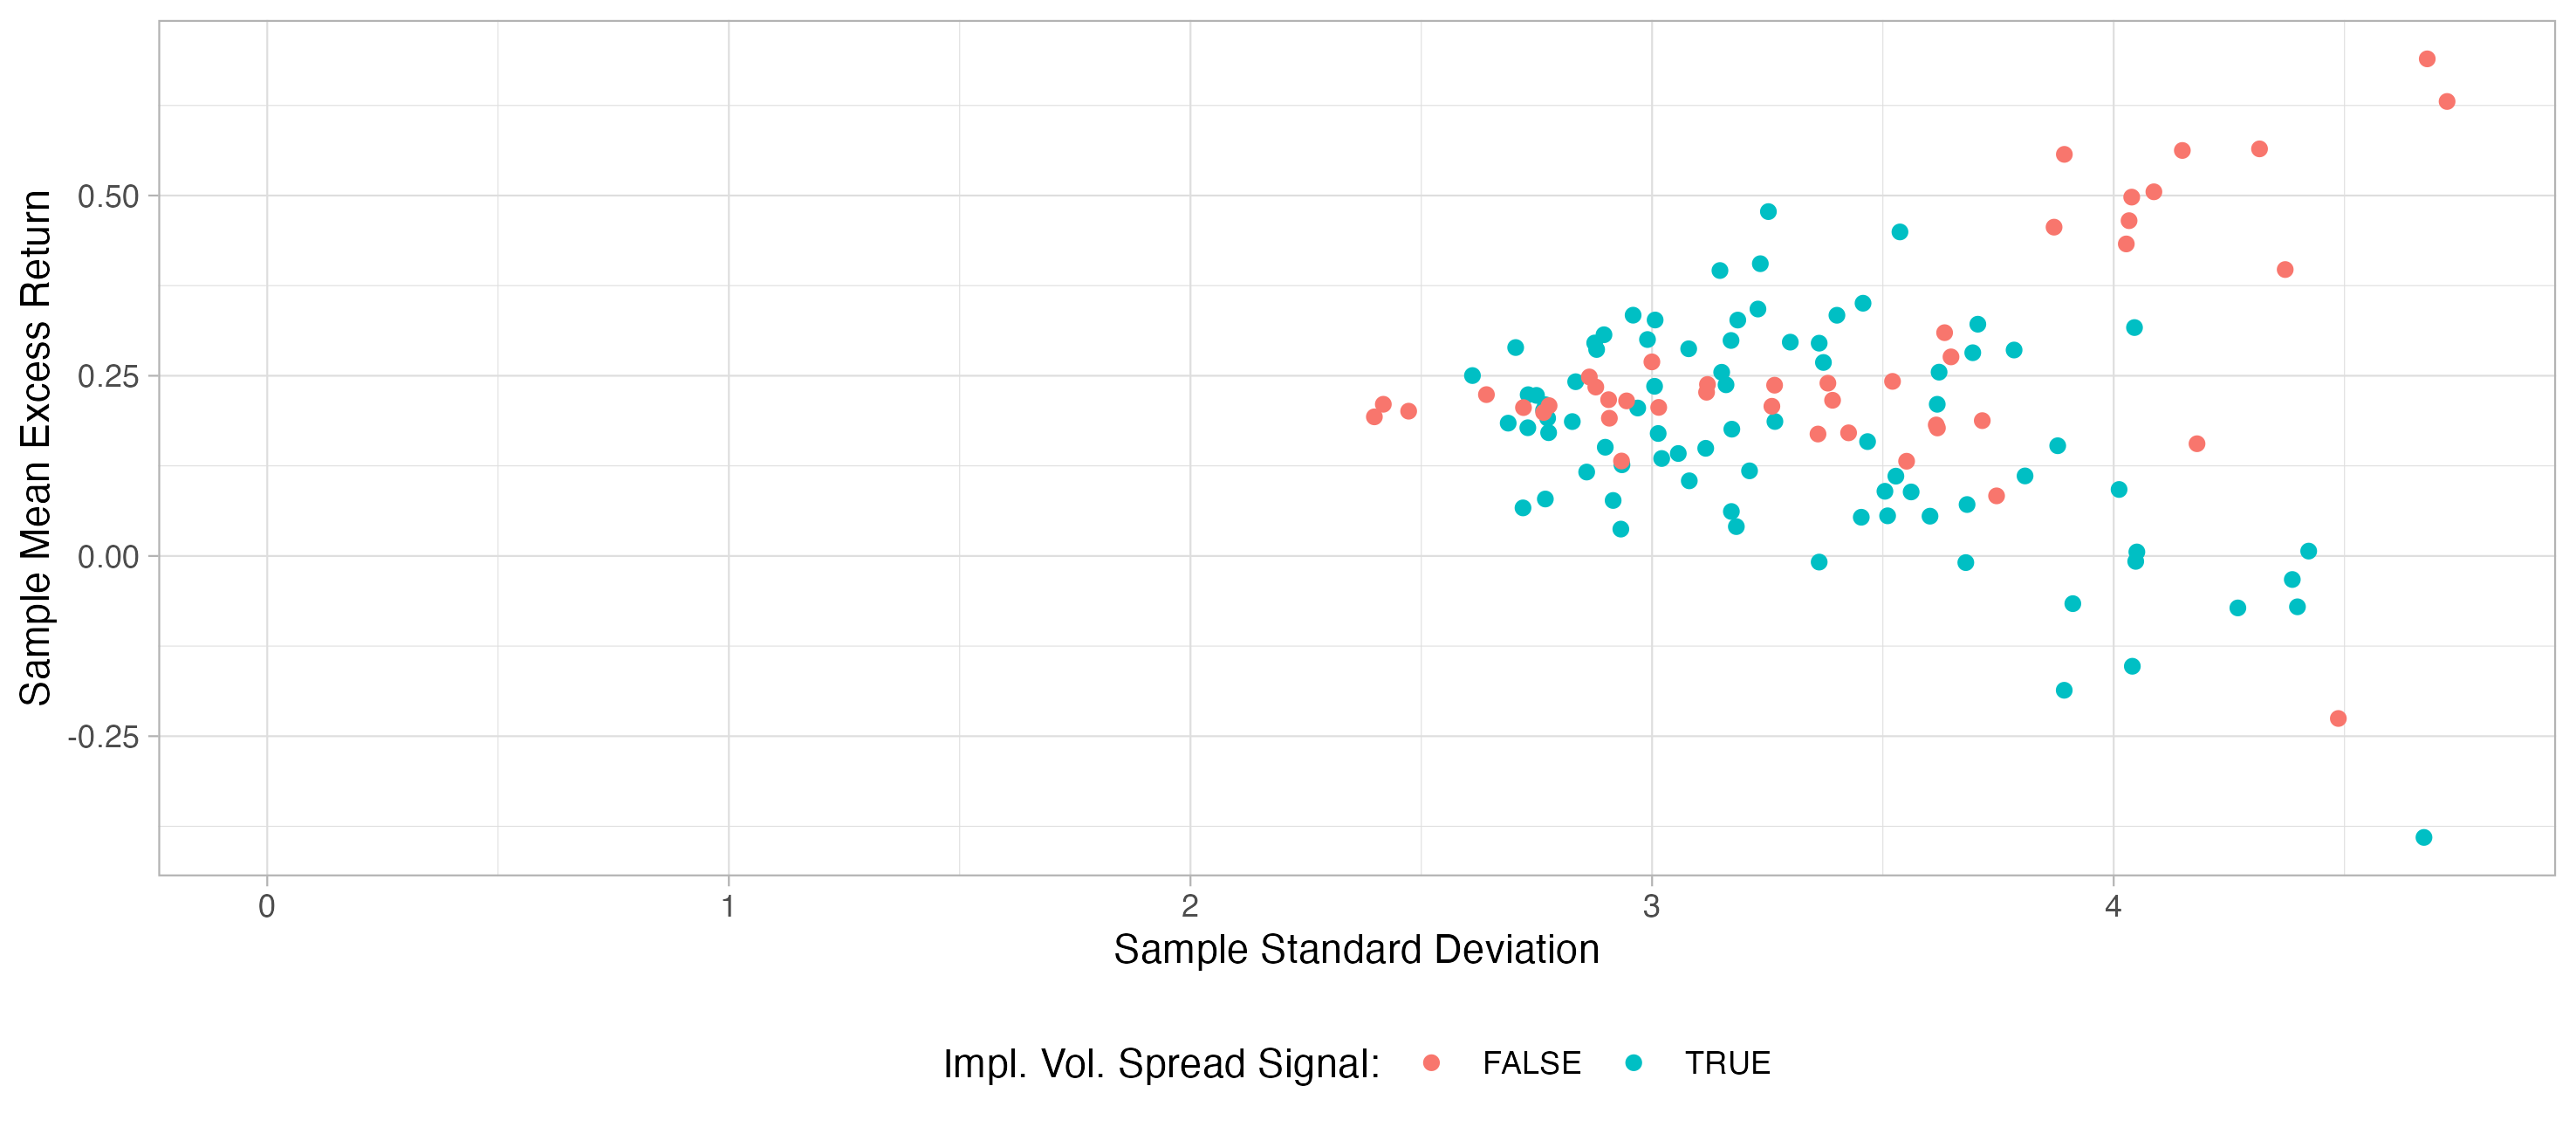
\includegraphics[width=0.75\textwidth]{./Plots/meanstd_efffrontier_entireperiod_9.png}} \\
		\subfloat[Efficient Frontier]{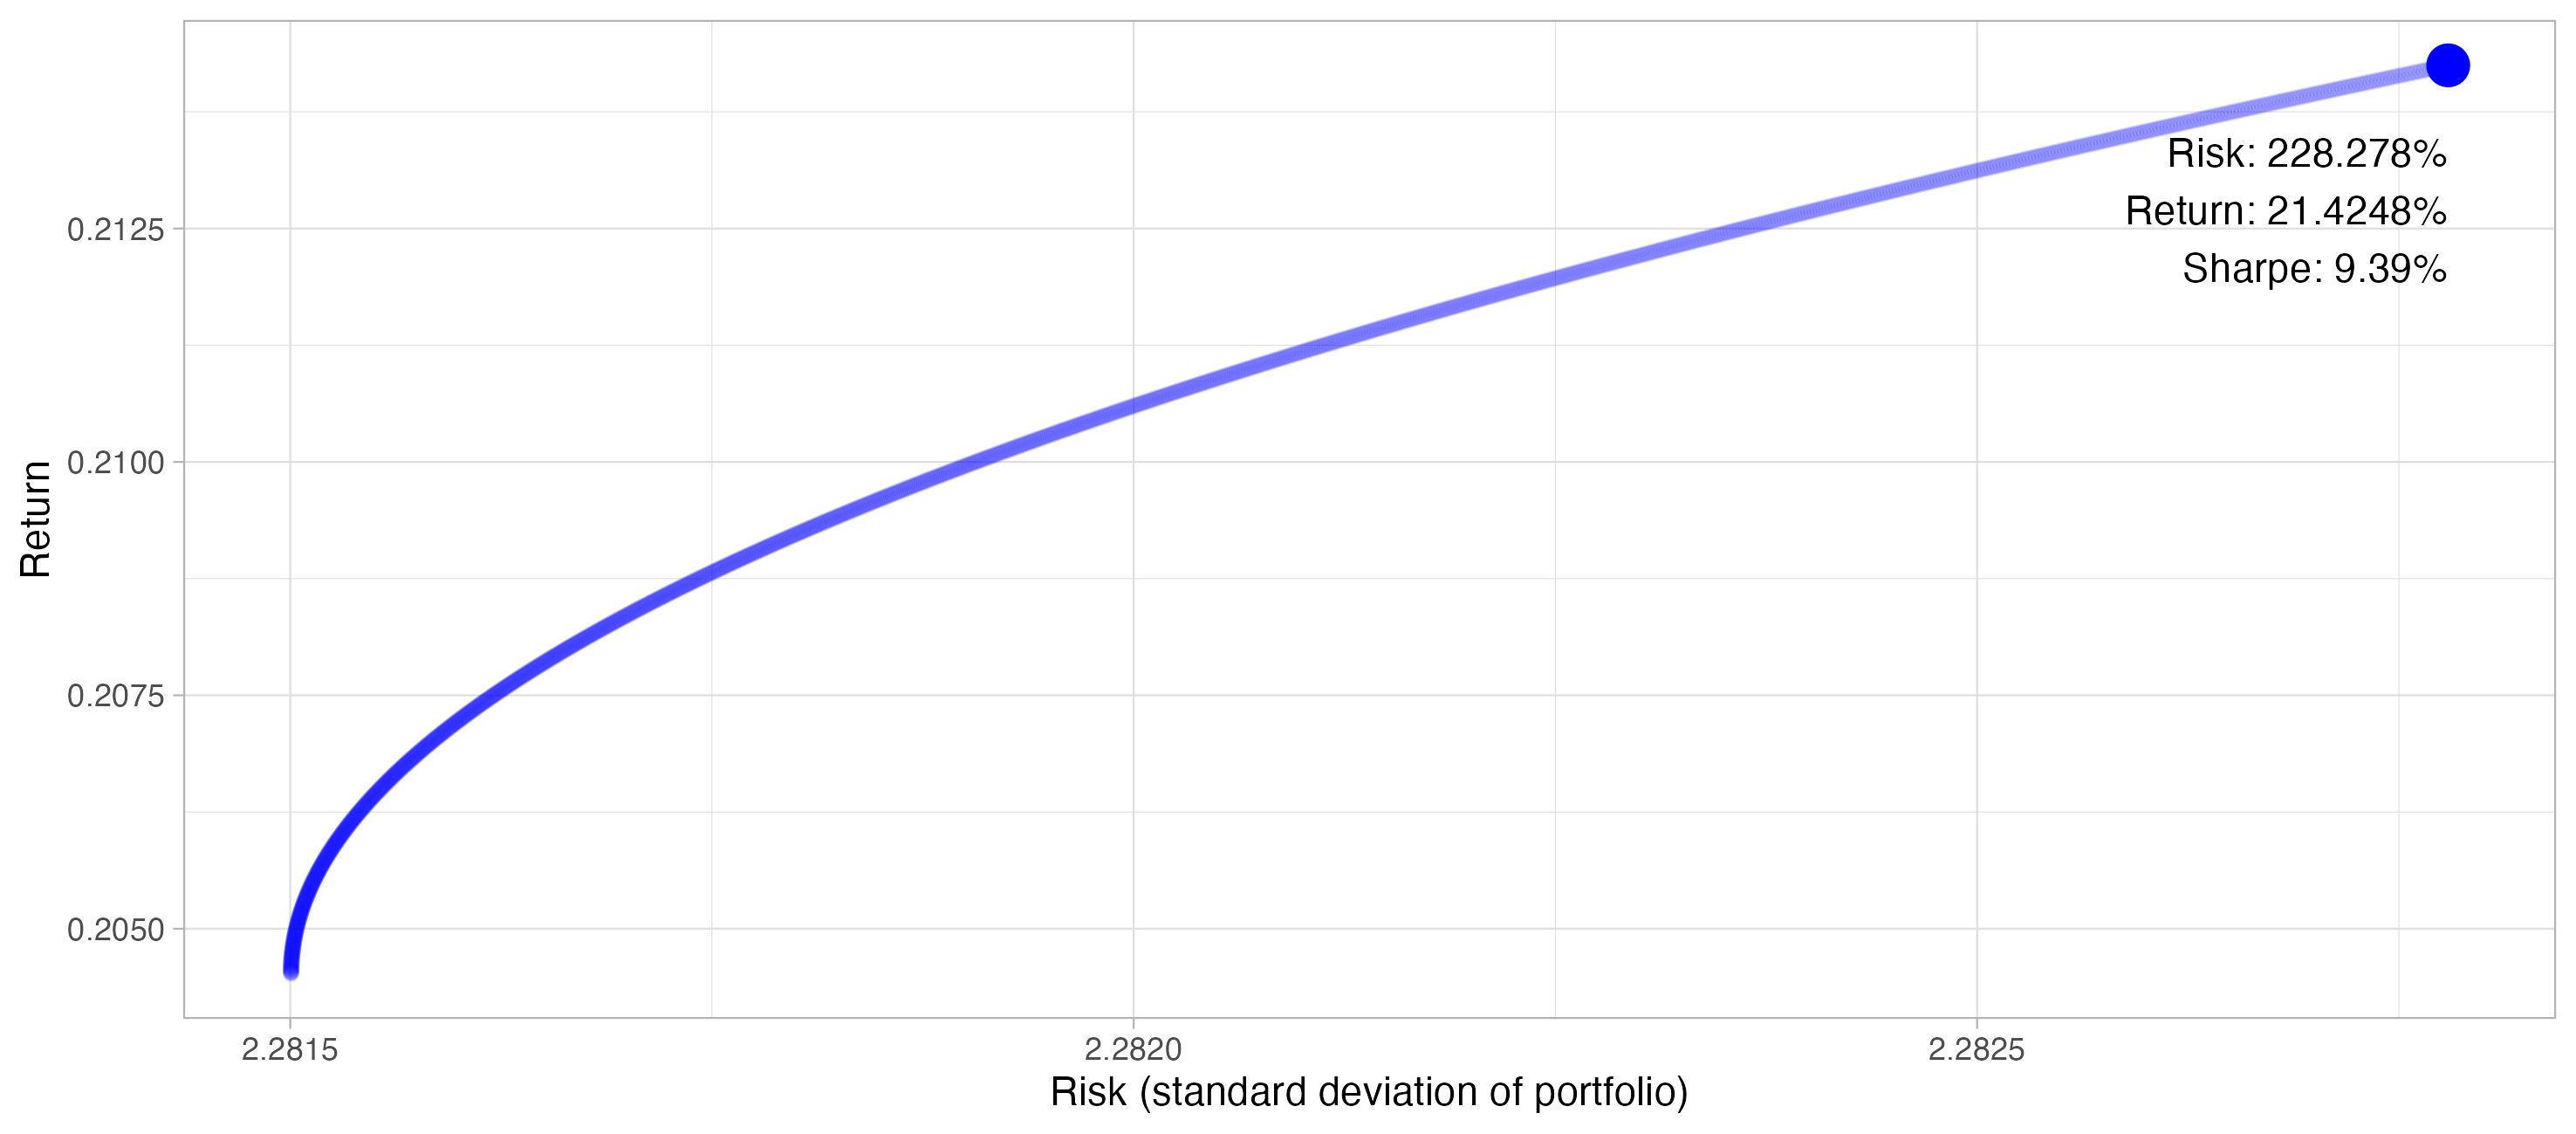
\includegraphics[width=0.75\textwidth]{./Plots/efficientfrontier_entireperiod_9.png}} \\
	\end{tabular}

	{\small Note: The returns are reported as the mean and standard deviation of each portfolio across the entire sample period. The x-axis denotes the standard deviation, and the y-axis denotes the excess weekly return. The first subfigure is colored according to the origin of the portfolios, turquoise for the implied volatility spread and orange for the Fama-French 5 times 5 portfolios on size and value. The ScenarioID is 9.}

	\label{fig:eff_frontier_9}
	
\end{figure}

When plotting the portfolios' mean and standard deviation within the sample period against the one incurred by the Fama-French portfolios in Figure \ref{fig:eff_frontier_9} subfigure (A) the portfolios form a distinct pattern. The Fama-French portfolios show an upwards trend of a higher standard deviation warrants a higher return, whereas the implied volatility spread portfolios show a sligthly more blurred picture, with a slight downward trend. 

A rational investor  would, however, not only let themselves be guided by the isolated mean and standard deviation of a portfolio, but instead evaluate it in the context of their existing portfolios. So in Figure \ref{fig:eff_frontier_9} subfigure (B) I have estimated the efficient frontier upon these 125 portfolios from above, and found identified the point upon the efficient frontier which provides the highest Sharpe Ratio. 

Figure \ref{fig:eff_frontier_9} does not, however, show how much to invest in the individual portfolios, which gives rise to the following analysis of the allocation to each portfolio given differing allocation constraints. 

The argument as to why the allocation constraints follow from a rational investor, who of course will only invest in the portfolio upon the efficient frontier with the highest Sharpe ratio, and then allocate their funds between the risky portfolio of assets and the risk free rate to satisfy their risk aversion. 

A rational investor might argue against forming the portfolios without any allocation constraints towards the individual portfolios. They could assume that exposure to only one particular portfolio on a subset of assets would not provide them with the diversification they desire. Therefore, allocation constraints raging from 0.05 to 0.5 must be evaluated, and the investor should then choose which of these combinations that provide them with sufficient diversification in their eyes. 

This is the reason as to a consideration of the different optimal allocation splits of the portfolio with the highest Sharpe Ratio given a range of allocation constraints for the individual portfolio. The results are shown in Figure \ref{fig:optimalloc}. 

\begin{figure}
	\centering
	
	\caption[Optimal Allocation]{Optimal Allocation given Allocation Constraints, in combination with FF5x5}
	\label{fig:optimalloc}
	
	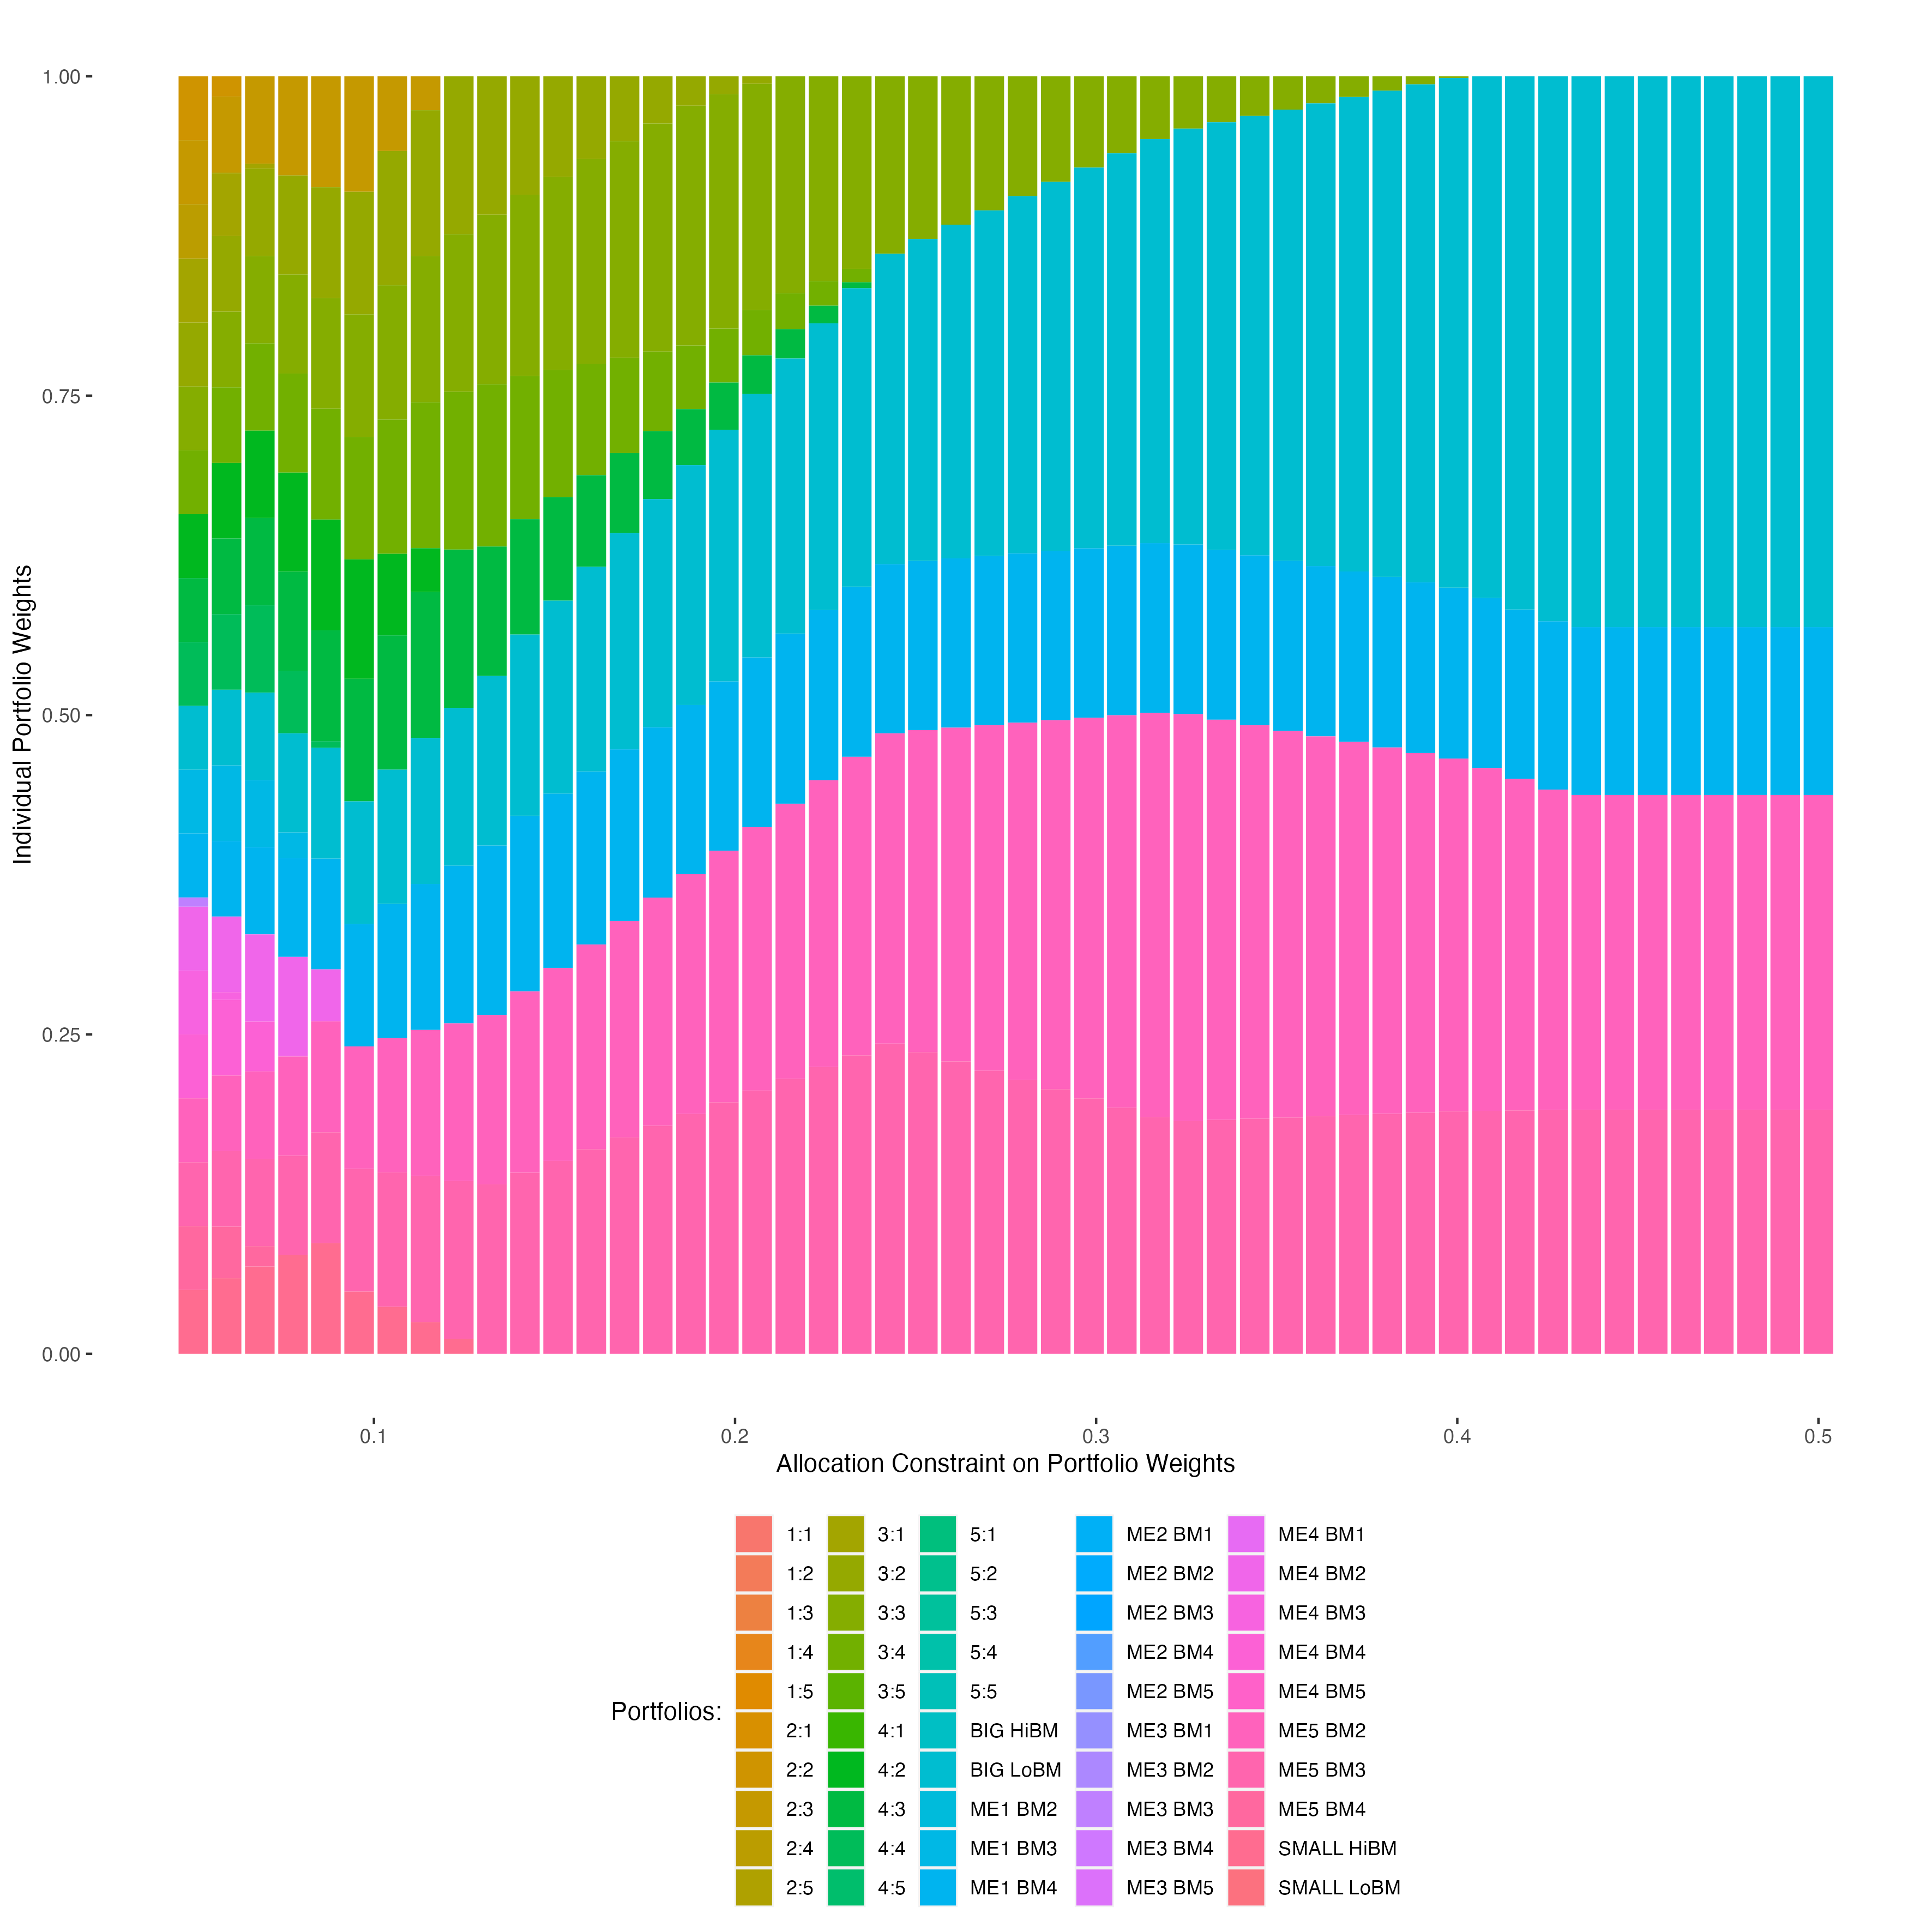
\includegraphics[width=0.95\textwidth]{./Plots/optimalallocation_SharpeRatio_entireperiod_2.png}
	
	{\small Note: The figure shows different investment structures given allocation constraints towards investment in the individual portfolio. All optimal portfolios are the combined portfolio with the highest Sharpe Ratio. The optimal allocation is calculated using shorting constraints. The ScenarioID is 2.}
\end{figure}


% Efficient Frontier

% Optimal Allocation + 25 portfolios from FF



%\subsection{Conclusion}
% – Conclusion
